\section{Architecture}

The basic components of \eTrice{} are depicted in the following diagram.

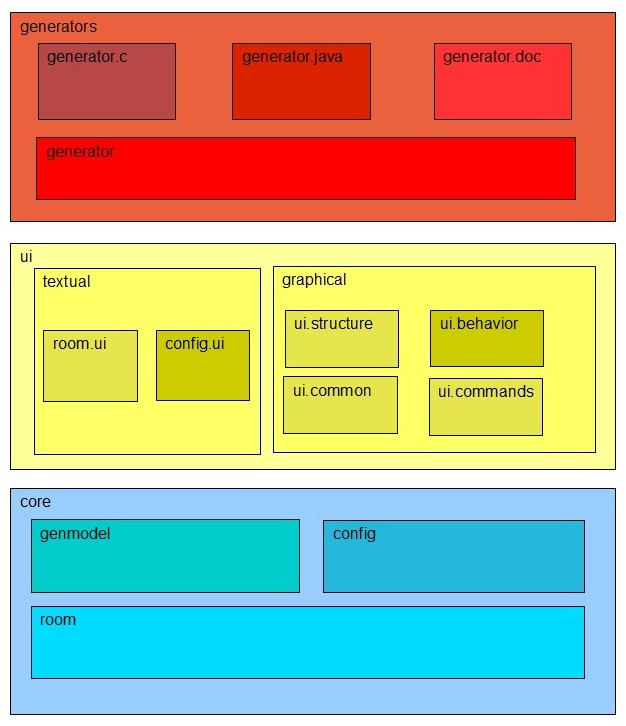
\includegraphics[scale=0.5]{images/200-components.jpg}

Additional to that the \eTrice{} project comprises runtime libraries and unit tests which are treated in 
subsequent sections.

\subsection{Editor and Generator Components}

\begin{itemize}
\item core

\begin{itemize}
\item core.common is an Xtext based language which serves as a base for other \eTrice{} languages.
It consists of the plug-ins
\texttt{org.eclipse.etrice.core.common} and
\texttt{org.eclipse.etrice.core.common.ui}.
The base grammar defines recurring items like numbers with literals, annotations and the like.
\item core.fsm is an Xtext based language that defines state machines in an abstract way.
It consists of the plug-ins
\texttt{org.eclipse.etrice.core.fsm} and
\texttt{org.eclipse.etrice.core.fsm.ui}.
The FSM language is abstract and has to be embedded in a model that defines containers for the state machine
with interface items (e.g. ROOM ports or Franca interfaces) and messages.
The ROOM grammar of \eTrice{} is derived from this grammar.
\item core.room is an Xtext based language called ROOM. It consists of the plug-ins
\texttt{org.eclipse.etrice.core.room} and
\texttt{org.eclipse.etrice.core.room.ui}. ROOM is the basic modeling language of \eTrice{}.
\item core.config is an Xtext based language called Config. It consists of the plug-ins
\texttt{org.eclipse.etrice.core.config} and
\texttt{org.eclipse.etrice.core.config.ui}. Config is a language designed for the data configuration of model 
\item core.etphys is an Xtext based language called etPhys. It consists of the plug-ins
\texttt{org.eclipse.etrice.core.etphys} and
\texttt{org.eclipse.etrice.core.etphys.ui}. etPhys is a language designed for the description of physical systems
onto which the logical ROOM systems are deployed.
\item core.etmap is an Xtext based language called etMap. It consists of the plug-ins
\texttt{org.eclipse.etrice.core.etmap} and
\texttt{org.eclipse.etrice.core.etmap.ui}. etMap is a language designed for the mapping of logical
to physical systems.
\item core.genmodel.fsm is an EMF based aggregation layer for finite state machines. It consists of the plugin 
\texttt{org.eclipse.etrice.core.genmodel.fsm}. A \texttt{ModelComponent} can be transformed into a \texttt{ExpandedModelComponent} which is an
explicit version of the state machine with all the inherited items contained.
\item core.genmodel is an EMF based aggregation layer for Room models. It consists of the plugin 
\texttt{org.eclipse.etrice.core.genmodel}. A Room model can be transformed into a genmodel which allows 
easy access to implicit relations of the Room model.
\end{itemize}

\item ui
\begin{itemize}
\item textual
\begin{itemize}

\item fsm.ui is the ui counterpart of core.fsm.  It consists of the plug-in 
\texttt{org.eclipse.etrice.core.fsm.ui}. This plug-in realizes IDE concepts like content assist, error 
markers and navigation by hyper links for the FSM language.
\item room.ui is the ui counterpart of core.room.  It consists of the plug-in 
\texttt{org.eclipse.etrice.core.room.ui}. This plug-in realizes IDE concepts like content assist, error 
markers and navigation by hyper links for the Room language.
\item config.ui is the ui counterpart of core.config.  It consists of the plug-in 
\texttt{org.eclipse.etrice.core.config.ui}. This plug-in realizes IDE concepts like content assist, error 
markers and navigation by hyper links for the Config language.
\item etphys.ui is the ui counterpart of core.etphys.  It consists of the plug-in 
\texttt{org.eclipse.etrice.core.etphys.ui}. This plug-in realizes IDE concepts like content assist, error 
markers and navigation by hyper links for the etPhys language.
\item etmap.ui is the ui counterpart of core.etmap.  It consists of the plug-in 
\texttt{org.eclipse.etrice.core.etmap.ui}. This plug-in realizes IDE concepts like content assist, error 
markers and navigation by hyper links for the etPhys language.
\end{itemize}

\item graphical
\begin{itemize}
\item ui.common.base is a set of common code for the diagram editors. It consists of the plug-in 
\texttt{org.eclipse.etrice.ui.common.base}. It depends only on the FSM part but not on ROOM.
\item ui.common is a set of common code for the two diagram editors. It consists of the plug-in 
\texttt{org.eclipse.etrice.ui.common}.
\item ui.commands encapsulates some commands related to the navigation between \eTrice{} editors. It consists 
of the plug-in \texttt{org.eclipse.etrice.ui.commands}.
\item ui.structure is the Graphiti based editor for the Actor structure. It consists of the plug-in 
\texttt{org.eclipse.etrice.ui.structure}.
\item ui.behavior.fsm is implementing the major part for the graphical state machine editor. It consists of the plug-in 
\texttt{org.eclipse.etrice.ui.behavior.fsm}. All property dialogs are handled in an abstract way
using a factory.
\item ui.behavior is the Graphiti based editor for the Actor behavior. It consists of the plug-in 
\texttt{org.eclipse.etrice.ui.behavior}. It utilizes the ui.behavior.fsm and provides concrete property dialogs.
\end{itemize}
\end{itemize}

\item generators
\begin{itemize}
\item generator.fsm is a set of general classes and language independent parts of all generators. It consists 
of the plug-in \textit{org.eclipse.etrice.generator.fsm}. It depends only on FSM but not on ROOM.
\item generator is a set of general classes and language independent parts of all generators. It consists 
of the plug-in \textit{org.eclipse.etrice.generator}.
\item generator.c is the generator for the ANSI-C target language. It consists of the plug-in 
\texttt{org.eclipse.etrice.generator.c}.
\item generator.cpp is the generator for the C++ target language. It consists of the plug-in 
\texttt{org.eclipse.etrice.generator.cpp}.
\item generator.java is the generator for the Java target language. It consists of the plug-in 
\texttt{org.eclipse.etrice.generator.java}.
\item generator.doc is the generator for the model documentation. It consists of the plug-in 
\texttt{org.eclipse.etrice.generator.doc}.
\end{itemize}
\end{itemize}

\subsection{The Abstract Finite State Machine Concept}

\eTrice{} comes with an easy to re-use concept of hierarchical finite state machines (FSM for short).
A powerful inheritance concept is used and there is also state machine validation based on
semantic rules for messages and abstract execution available.

State machines are an integral part of the ROOM language. But they can also be used independently from that using

\begin{itemize}

\item for the model part
\begin{itemize}
\item \texttt{org.eclipse.etrice.core.common}
\item \texttt{org.eclipse.etrice.core.fsm}
\item \texttt{org.eclipse.etrice.core.genmodel.fsm}
\end{itemize}

\item graphical state machine editor
\begin{itemize}
\item \texttt{org.eclipse.etrice.core.common.ui}
\item \texttt{org.eclipse.etrice.core.fsm.ui}
\item \texttt{org.eclipse.etrice.core.ui.common.base}
\item \texttt{org.eclipse.etrice.core.ui.common}
\end{itemize}

\item base classes for code generation
\begin{itemize}
\item \texttt{org.eclipse.etrice.generator.fsm}
\end{itemize}

\item validation by abstract execution
\begin{itemize}
\item \texttt{org.eclipse.etrice.abstractexec.behavior}
\end{itemize}

\end{itemize}

The first three parts have to be used by concrete implementations that implement the abstract interface.
\eTrice{} itself uses the abstract FSMs in exactly this way.

\subsubsection{Extending the FSM Model}

The \eTrice{} FSM model has to be embedded in a model that introduces components, interfaces and messages.
We recommend to use a new Xtext language with a grammar derived from the FSM grammar.
This grammar has to specify a component derived from the \texttt{ModelComponent} of the FSM model.
It further has to introduce concrete realizations of interface items derived from \texttt{AbstractInterfaceItem}.
The interface item is an object contained in a component that has a name (role) and holds a reference to some kind of interface of the
component (like a Franca interface or a ROOM protocol).
Finally a concrete message type derived from an \texttt{EObject} has to be defined. The minimal requirement is that this concrete message
has an attribute called 'name' of type String.

The minimal interface to be implemented consists of
\begin{itemize}
	\item for the concrete interface item
	\begin{itemize}
		\item \texttt{EList<EObject> getAllIncomingAbstractMessages()}
		\item \texttt{EList<EObject> getAllOutgoingAbstractMessages()}
		\item \texttt{ProtocolSemantics getSemantics()}
	\end{itemize}
	\item for the concrete model component
	\begin{itemize}
		\item \texttt{EList<AbstractInterfaceItem> getAbstractInterfaceItems} -- the interface items contained in this model component
		\item \texttt{EList<AbstractInterfaceItem> getAllAbstractInterfaceItems} -- all interface items including inherited ones
		\item \texttt{String getComponentName()} -- should return the name of the model component
	\end{itemize}
\end{itemize}

\subsubsection{Extending the State Machine Editor}

The concrete state machine editor minimally needs to define
\begin{itemize}
\item the editor class itself by deriving it from the \texttt{AbstractFSMEditor}
\item a diagram type provider (which may derive from \texttt{AbstractDiagramTypeProvider})
\item a Google Guice module with bindings for
	\begin{itemize}
	\item \texttt{IFSMDialogFactory}
	\item \texttt{DiagramAccessBase}
	\item \texttt{IBehaviorQuickfixProvider}
	\item \texttt{IResourceSetProvider}
	\end{itemize}
\item concrete implementations of all property dialogs the \texttt{IFSMDialogFactory} produces
\end{itemize}


\subsection{Runtimes}

Currently \eTrice{} ships with a C and a Java runtime. The C++ runtime is still a prototype.
The runtimes are libraries written in the target 
language against which the generated code is compiled.

\subsection{Unit Tests}

Most plug-ins and other parts of the code have related unit tests.

\section{Component Overview}

\subsection{Room Language Overview}

We assume that the reader is familiar with the Xtext concepts. So we concentrate on the details of our 
implementation that are worth to be pointed out.

\subsubsection{Model Tweaks}

All language EMF models of \eTrice{} are inferred from their respective grammar.
However, this powerful mechanism has to be tweaked in some places.

In order to do so post processors are added that are invoked by the Xtext framework on language generation.
This is done for the FSM language by \textit{/org.eclipse.etrice.core.fsm/src/org/eclipse/etrice/core/fsm/postprocessing/ImplPostprocessor.xtend}.

The following parts of the model are changed or added:
\begin{itemize}
\item an operation \texttt{getName} is added to the \texttt{State} class
\item an operation \texttt{getName} is added to the \texttt{StateGraphItem} class
\item an operation \texttt{getSemantics} is added to the \texttt{AbstractInterfaceItem}
\item an operation \texttt{getAllIncomingAbstractMessages} is added to the \texttt{AbstractInterfaceItem}
\item an operation \texttt{getAllOutgoingAbstractMessages} is added to the \texttt{AbstractInterfaceItem}
\item an interface class \texttt{IInterfaceItemOwner} is added
\item an operation \texttt{getAbstractInterfaceItems} is added to the \texttt{AbstractInterfaceItem}
\item an operation \texttt{getAllAbstractInterfaceItems} is added to the \texttt{AbstractInterfaceItem}
\item \texttt{IInterfaceItemOwner} is made a super class of \texttt{ModelComponent}
\end{itemize}
All but the first two items in the list are part of the abstract FSM definition and are used to interface
to the model embedding the FSM language, e.g. ROOM.

For the ROOM language the post processor is
\textit{/org.eclipse.etrice.core.room/src/org/eclipse/etrice/core/RoomPostprocessor.ext}.

The following parts of the model are changed or added:
\begin{itemize}
\item the default \texttt{multiplicity} of the \texttt{Port} is set to 1
\item the operation \texttt{isReplicated} is added to the \texttt{Port}
\item the default \texttt{multiplicity} of the \texttt{ActorRef} is set to 1
\item an operation \texttt{getGeneralProtocol} is added to the \texttt{InterfaceItem}
\item an operation \texttt{getSemantics} is added to the \texttt{InterfaceItem}
\item an operation \texttt{getAllIncomingAbstractMessages} is added to the \texttt{InterfaceItem}
\item an operation \texttt{getAllOutgoingAbstractMessages} is added to the \texttt{InterfaceItem}
\item an operation \texttt{getExternalEndPorts} is added to the \texttt{ActorClass}
\item an operation \texttt{getRelayPorts} is added to the \texttt{ActorClass}
\item an operation \texttt{getImplementedSPPs} is added to the \texttt{ActorClass}
\item an operation \texttt{getActorBase} is added to the \texttt{ActorClass}
\item an operation \texttt{getComponentName} is added to the \texttt{ActorClass}
\item an operation \texttt{getAbstractInterfaceItems} is added to the \texttt{ActorClass}
\item an operation \texttt{getAllAbstractInterfaceItems} is added to the \texttt{ActorClass}
\item an operation \texttt{getStructureClass} is added to the \texttt{ActorContainerRef}
\item an operation \texttt{toString} is added to the \texttt{RefPath}
\item for attribute \texttt{idx} of \texttt{RefSegment} the default is changed to -1
\item an operation \texttt{toString} is added to the \texttt{RefSegment}
\item an operation \texttt{getLiteralValue} is added to the \texttt{EnumLiteral}
\item an operation \texttt{getFullName} is added to the \texttt{EnumLiteral}
\end{itemize}

\subsubsection{Imports by URI Using Namespaces}

The import mechanism employed is based on URIs. This is configured for one part in the GenerateRoom.mwe2 
model workflow by setting the fragments ImportURIScopingFragment and ImportUriValidator). For the other 
part it is configured in the Guice modules by binding
\begin{itemize}
\item \texttt{PlatformRelativeUriResolver} -- this class tries to convert the import URI into a platform 
relative URI. It also replaces environment variables written in \${} with their respective values.
\item \texttt{ImportedNamespaceAwareLocalScopeProvider} -- this is a standard scope provider which is 
aware of namespaces
\item \texttt{GlobalNonPlatformURIEditorOpener} -- this editor opener tries to convert general URIs into 
platform URIs because editors can only open platform URIs
\item \texttt{ImportAwareHyperlinkHelper} -- turns the URI part of an import into a navigatable hyper link
\end{itemize}

\subsubsection{Naming}

Two classes provide object names used for link resolution and for labels.
The \texttt{RoomNameProvider} provides frequently used name strings, some of them are hierarchical like 
State paths.
The \texttt{RoomFragmentProvider} serves a more formal purpose since it provides a link between EMF models 
(as used by the diagram editors) and the textual model representation used by Xtext.

\subsubsection{Helpers}

The \texttt{RoomHelpers} class provides a great deal of static methods that help retrieve frequently used 
information from the model.
Among many, many others
\begin{itemize}
\item \texttt{getAllEndPorts(ActorClass)} - returns a list of all end ports of an actor class including 
inherited ones
\item \texttt{getInheritedActionCode(Transition, ActorClass)} - get the inherited part of a transition's 
action code
\item \texttt{getSignature(Operation)} - returns a string representing the operation signature suited for 
a label
\end{itemize}

\subsubsection{Validation}

Validation is used from various places. Therefore all validation code is accumulated in the 
@ValidationUtil@ class. All methods are static and many of them return a Result object which contains 
information about the problem detected as well as object and feature as suited for most validation purposes.

\subsection{Config Language Overview}

\subsubsection{Model Tweaks}

A couple of operations are added to the ConfigModel
\begin{itemize}
\item \texttt{getActorClassConfigs}
\item \texttt{getActorInstanceConfigs}
\item \texttt{getProtocolClassConfigs}
\item \texttt{getSubSystemConfigs}
\end{itemize}

\subsubsection{Imports by URI Using Namespaces}

Imports are treated like in Room language, section \textit{Imports by URI Using Namespaces}.

\subsubsection{Util}

A set of static utility methods can be found in the \texttt{ConfigUtil} class.

\subsection{Aggregation Layer Overview}

The \eTrice{} Generator Model (genmodel.fsm and genmodel) serves as an aggregation layer. Its purpose is to allow easy access 
to information which is implicitly contained in the Room model but not simple to retrieve.
Examples of this are the state machine with inherited items or a list of all triggers active at a state in 
the order in which they will be evaluated or the actual peer port of an end port (following bindings 
through relay ports).

The lower level \texttt{FSMGeneratorModelBuilder} takes a \texttt{ModelComponent} and returns a \texttt{ExpandedModelComponent} which
has the inheritance hierarchy of the state machine collapsed into one state machine.
This lower level generator model only depends on general parts and doesn't refer to the ROOM model.

The higher level Generator Model includes the FSM Generator Model.
It is created from a list of Room models by a call of the

\begin{verbatim}createGeneratorModel(List<RoomModel>, boolean)\end{verbatim}

method of the \texttt{GeneratorModelBuilder} class.

The \texttt{Root} object of the resulting Generator Model provides chiefly two things:
\begin{itemize}
\item a tree of instances starting at each \texttt{SubSystem} with representations of each 
\texttt{ActorInstance} and \texttt{PortInstance}
\item for each \texttt{ActorClass} a corresponding \texttt{ExpandedActorClass} with an explicit state 
machine containing all inherited state graph items
\end{itemize}

\subsubsection{The Instance Model}

The instance model allows easy access to instances including their unique paths and object IDs. Also it is 
possible to get a list of all peer port instances for each port instance without having to bother about 
port and actor replication.

\subsubsection{The Expanded Model Component}

The expanded model component contains, as already mentioned, the complete state machine of the model component. 
This considerably simplifies the task of state machine generation. Note that the generated code always 
contains the complete state machine of an actor. I.e. no target language inheritance is used to implement 
the state machine inheritance.
Furthermore the \texttt{ExpandedModelComponent} gives access to
\begin{itemize}
\item \texttt{getIncomingTransitions(StateGraphNode)} -- the set of incoming transition of a 
\texttt{StateGraphNode} (\texttt{State}, \texttt{ChoicePoint} or \texttt{TransitionPoint})
\item \texttt{getOutgoingTransitions(StateGraphNode)} -- the set of outgoing transition of a 
\texttt{StateGraphNode}
\item \texttt{getActiveTriggers(State)} -- the triggers that are active in this \texttt{State} in the 
order they are evaluated
\end{itemize}

\subsubsection{The Expanded Actor Class}

The \texttt{ExpandedActorClass} is derived from the \texttt{ExpandedModelComponent} and adds only minor new features.
\begin{itemize}
\item \texttt{getActorClass()} -- for convenience to avoid casts of the \texttt{ModelComponent} to an \texttt{ActorClass} 
\item \texttt{getVarDeclData(Transition)} -- for convenience to avoid casts to \texttt{VarDecl}
\end{itemize}

\subsubsection{Transition Chains}

By transition chains we denote a connected subset of the (hierarchical) state machine that starts with a 
transition starting at a state and continues over transitional state graph nodes (choice points and 
transition points) and continuation transitions until a state is reached. In general a transition chain 
starts at one state and ends in several states (the chain may branch in choice points).
A \texttt{TransitionChain} of a transition is retrieved by a call of \texttt{getChain(Transition)} of the 
\texttt{ExpandedActorClass}.
The \texttt{TransitionChain} accepts an \texttt{ITransitionChainVisitor} which is called along the chain 
to generate the action codes of involved transitions and the conditional statements arising from the 
involved choice points. 

\subsection{Generator Overview}

There is one plug-in that consists of base classes and some generic generator parts which are re-used by 
all language specific generators
 
\subsubsection{Base Classes and Interfaces}

We just want to mention the most important classes and interfaces.
Some of them can be found in the \texttt{org.eclipse.etrice.generator.fsm} and th rest
in \texttt{org.eclipse.etrice.generator}.

\begin{itemize}
\item \begin{flushleft}\texttt{ITranslationProvider} --- this interface is used by the 
\texttt{DetailCodeTranslator} for the language dependent translation of e.g. port.message() notation in 
detail code\end{flushleft}
\item \texttt{AbstractGenerator} --- concrete language generators should derive from this base class
\item \begin{flushleft}\texttt{DefaultFSMTranslationProvider} and \texttt{DefaultTranslationProvider} --- a stub implementation of 
\texttt{IFSMTranslationProvider} and \texttt{ITranslationProvider} from which clients may derive\end{flushleft}
\item \texttt{Indexed} --- provides an indexed iterable of a given iterable
\item \texttt{GeneratorBaseModule} --- a Google Guice module that binds a couple of basic services. 
Concrete language generators should use a module that derives from this
\end{itemize}

\subsubsection{Generic Generator Parts}

The generic generator parts provide code generation blocks on a medium granularity. The language dependent 
top level generators embed those blocks in a larger context (file, class, ...). Language dependent low 
level constructs are provided by means of an \texttt{ILanguageExtension}. This extension and other parts 
of the generator be configured using Google Guice dependency injection.

\paragraph{GenericActorClassGenerator}

The \texttt{GenericActorClassGenerator} generates constants for the interface items of a actor. Those 
constants are used by the generated state machine.

\paragraph{GenericProtocolClassGenerator}

The \texttt{GenericProtocolClassGenerator} generates message ID constants for a protocol.

\paragraph{GenericStateMachineGenerator}

\begin{flushleft}The \texttt{GenericStateMachineGenerator} generates the complete state machine 
implementation. The skeleton of the generated code is\end{flushleft}

\begin{itemize}
\item definition state ID constants
\item definition of transition chain constants
\item definition of trigger constants
\item entry, exit and action code methods
\item the \texttt{exitTo} method 
\item the \texttt{executeTransitionChain} method
\item the \texttt{enterHistory} method
\item the \texttt{executeInitTransition} method
\item the \texttt{receiveEvent} method
\end{itemize}

The state machine works as follows. The main entry method is the \\ \texttt{receiveEvent} method. This is 
the case for both, data driven (polled) and event driven state machines. Then a number of nested 
switch/case statements evaluates trigger conditions and derives the transition chain that is executed. If 
a trigger fires then the \texttt{exitTo} method is called to execute all exit codes involved. Then the 
transition chain action codes are executed and the choice point conditions are evaluated in the 
\texttt{executeTransitionChain} method. Finally the history of the state where the chain ends is entered 
and all entry codes are executed by \texttt{enterHistory}.

\subsubsection{The Java Generator}

The Java generator employs the generic parts of the generator. The \texttt{JavaTranslationProvider} is 
very simple and only handles the case of sending a message from a distinct replicated port: 
\texttt{replPort[2].message()}. Other cases are handled by the base class by returning the original text.

The \texttt{DataClassGen} uses Java inheritance for the generated data classes. Otherwise it is pretty 
much straight forward.

The \texttt{ProtocolClassGen} generates a class for the protocol with nested static classes for regular 
and conjugated ports and similar for replicated ports.

The \texttt{ActorClassGen} uses Java inheritance for the generated actor classes. So ports, SAPs and 
attributes and detail code methods are inherited. Not inherited is the state machine implementation.

\subsubsection{The ANSI-C Generator}

The C generator translates data, protocol and actor classes into structs together with a set of methods 
that operate on them and receive a pointer to those data (called \texttt{self} in analogy to the implicit 
C++ \texttt{this} pointer).
No dynamic memory allocation is employed. All actor instances are statically initialized.
One of the design goals for the generated C code was an optimized footprint in terms of memory and 
performance to be able to utilize modeling with ROOM also for tiny low end micro controllers.

\subsubsection{The Documentation Generator}

The documentation generator creates documentation in LaTex format which can be converted into PDF and many 
other formats.
